\documentclass[12pt]{amsart}
\usepackage[margin=0.5in]{geometry}     
\usepackage[section]{placeins}
\geometry{letterpaper}                   % ... or a4paper or a5paper or ... 
%\geometry{landscape}                % Activate for for rotated page geometry
%\usepackage[parfill]{parskip}    % Activate to begin paragraphs with an empty line rather than an indent
\usepackage{graphicx}
\usepackage{amssymb}
\usepackage{epstopdf}
\DeclareGraphicsRule{.tif}{png}{.png}{`convert #1 `dirname #1`/`basename #1 .tif`.png}
\newcommand{\tbf}{\textbf}
%%%%%%%%%%%%%%%%%%%%%%%%%%%%%%%%%%%%%%%%%%
%ignore everything before here

%lab number
\newcommand{\reportnumber}{2}

%%%%%%%%%%%%%%%%%%%%%%%%%%%%%%%%%%%%%%%%%%
%DO NOT ALTER
\title{ELEC  243: Lab Report \# \reportnumber}
\author{Carissa Livingston \& Fernando Ramirez}
\date{\today}
%%%%%%%%%%%%%%%%%%%%%%%%%%%%%%%%%%%%%%%%%%
%Document starts here
\begin{document}
	\maketitle
%%%%%%%%%%%%%%%%%%%%%%%%%%%%%%%%%%%%%%%%%%%
	\section{Summary}
%words about how awesome the lab was
%%%%%%%%%%%%%%%%%%%%%%%%%%%%%%%%%%%%%%%%%%%
	\section{Data and Analysis}

		%% For putting in a Table
		%\begin{table}[h]
		%\caption{Title} % title of Table
		%\centering  % used for centering table
		%\begin{tabular}{c c c c} % centered columns (4 columns)
		%\hline\hline                        %inserts double horizontal lines
		% % inserts table 
		%%heading
		%\hline                  % inserts single horizontal line
		%Data % [1ex] adds vertical space
		%\hline %inserts single line
		%\end{tabular}
		%\label{Table} % is used to refer this table in the text
		%\end{table}

		%% For putting in a figure
		%\begin{figure}
		%	\centering
		%	\includegraphics[width=4.2in]{figure/}
		%\end{figure}
		%% 
%%%%%%%%%%%%%%%%%%%%%%%%%%%%%%%%%%%%%%%%%%%
	\section{Experiment 2.1: The Oscilloscope and Function Generator}
	\subsection{Viewing Signals with the Oscilloscope}
		\tbf{What does pulling the red X1-X5 switch in the middle of the timebase's position knob do? What is the effect of changing the slope trigger control from "+" to "-"?}		\\ \\
		\tbf{Describe what happens when you change the vertical amplifier settings, or switch to uncalibrated mode.}\\ \\
	\subsection{Quantitative Measurements with the Oscilloscope}
		\tbf{Question 1: Why would we want to use the oscilloscope to measure a "DC" voltage? } \\ \\		
		\tbf{How does your calculated frequency of the signal (using the formula f=1/T) compare with the nominal frequency? } \\ \\
		\tbf{Question 2: The calibration output has no place for attaching the black ground (common) lead: why not? }		\\ \\
		\tbf{Sketch the calibration signal's waveform. What is its period? What is its frequency?  Does your measurement of the waveform's amplitude correspond to the stated value? }
%%%%%%%%%%%%%%%%%%%%%%%%%%%%%%%%%%%%%%%%%%%
	\section{Experiment 2.2 Electroacoustic Transducers}
	\subsection{Listening to a Signal}
		\tbf{What do you hear when you connect the output of the function generator to the speaker?  }\\ \\		
		\tbf{With the speaker still connected to the function generator (Step 3), is the voltage across the speaker still 5V (p-p)?  } \\ \\
		\tbf{Describe the nature of the sound change as you changed the function generator parameters (Step 4).}		\\ \\
	\subsection{Microphone}
		\tbf{Briefly describe the effects of the triggering and time sweep controls on the display of the microphone signal (Step 6).}		\\ \\
		\tbf{Sketch one or two of the more interesting waveshapes from speaking vowels (Step 8). What was the approximate frequency of your sustained vowel sound?}\\ \\
		\tbf{Is the waveform on the oscilloscope from your whistle sinusoidal?  }\\ \\		
		\tbf{Question 3: Based on your measurements of the loudspeaker sensitivity and the output of the microphone, would it be possible to produce an audible sound in the loudspeaker by connecting it directly to the microphone? }\\ \\
%%%%%%%%%%%%%%%%%%%%%%%%%%%%%%%%%%%%%%%%%%%
	\section{Experiment 2.3 Optoelectronic Transducers}
	\subsection{The Photodiode}
		\tbf{Note the voltage produced by the photodiode in room light, when you cover the photodiode with your hand, when you illuminate it with (a) the under-shelf florescent lamp and (b) the incandescent lamp.  Sketch the shape of the AC component of the waveform for each source. What is its amplitude and frequency? }	\\ \\	
		% For putting in a figure
		\begin{figure}
			\centering
			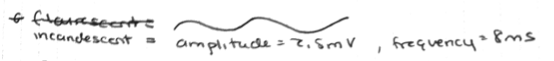
\includegraphics[width=6in]{figure/incan}
		\end{figure}
		% 
				% For putting in a figure
		\begin{figure}
			\centering
			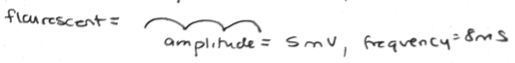
\includegraphics[width=6in]{figure/flour}
		\end{figure}
		% 
		change
		\tbf{Question 4: Explain the waveforms you observed above. }\\ \\
	\subsection{Measuring Photocurrent}
		\tbf{Specify the voltage and photocurrent measured using the same three light sources as in Part 1. }		\\ \\
	\subsection{Light Emitting Diode}
		\tbf{What is the voltage across the LED for supply voltages of 3, 4, and 5 volts. Comment on the relative LED brightness at each setting.}\\ \\		
		\tbf{At what excitation frequency does the appearance of steady glow from the LED stop and noticeable flicker begin?  }\\ \\
		\tbf{Question 5: How does the number you measured in the previous step relate to the frame rate of television and motion pictures? }\\ \\	
	\subsection{Optical Communication, Take 1}
		\tbf{Describe the waveform from the photodiode in response to the LED�s light. Is it what you would expect? }		\\ \\
		\tbf{Sketch the waveform from the photodiode for a triangle excitation of the LED.  Is it what you expected? Can you explain it? }\\ \\
		\tbf{What is the maximum separation of the LED and photodiode for which you can transmit a recognizable signal?}		\\ \\
%%%%%%%%%%%%%%%%%%%%%%%%%%%%%%%%%%%%%%%%%%%
	\section{Feedback}
\end{document}